\section{Informazioni Generali}

\begin{itemize}
	\item{\textbf{Luogo}}: Meeting Discord
	\item{\textbf{Data}}: \D
	\item{\textbf{Ora}}: 18:10 - 19:30
	\item{\textbf{Partecipanti del Gruppo}}:
	\begin{itemize}
		\item{\EP{};}
		\item{\FP{};}
		\item{\GC{};}
		\item{\LW{};}
		\item{\MG{};}
		\item{\MG{};}
		\item{\PV{}.}
	\end{itemize}
	\item{\textbf{Segretario}}: \GC{}
\end{itemize}

\section{Ordine del Giorno}
\begin{itemize}
	\item{Discussione sullo stato di avanzamento;}
	\item{Filtri e Likes da implementare nella WebApp;}
	\item{Coordinazione interna.}
\end{itemize}

\section{Resoconto}

\subsection{Stato di avanzamento del progetto}

Il prof. Vardanega ci ha inviato una comunicazione relativa al fatto che non ha più ricevuto nostre notizie in merito allo stato di avanzamento del progetto o di eventuali problematiche riscontrate. In questa occasione, abbiamo riflettuto sui problemi individuati nelle ultime settimane (sia tecnici che collaborativi) ed abbiamo cercato di riassumere tutto ciò in maniera concisa, per dare una risposta il più completa possibile alla comunicazione ricevuta.

Tuttavia, questa comunicazione ci ha permesso di discutere collettivamente su problematiche che non erano mai state trattate, come la coordinazione interna tra le diverse parti (Front-end e Back-end).  

A seguire la risposta integrale all'e-mail del prof. Vardanega.

\begin{figure}[H]
\centering
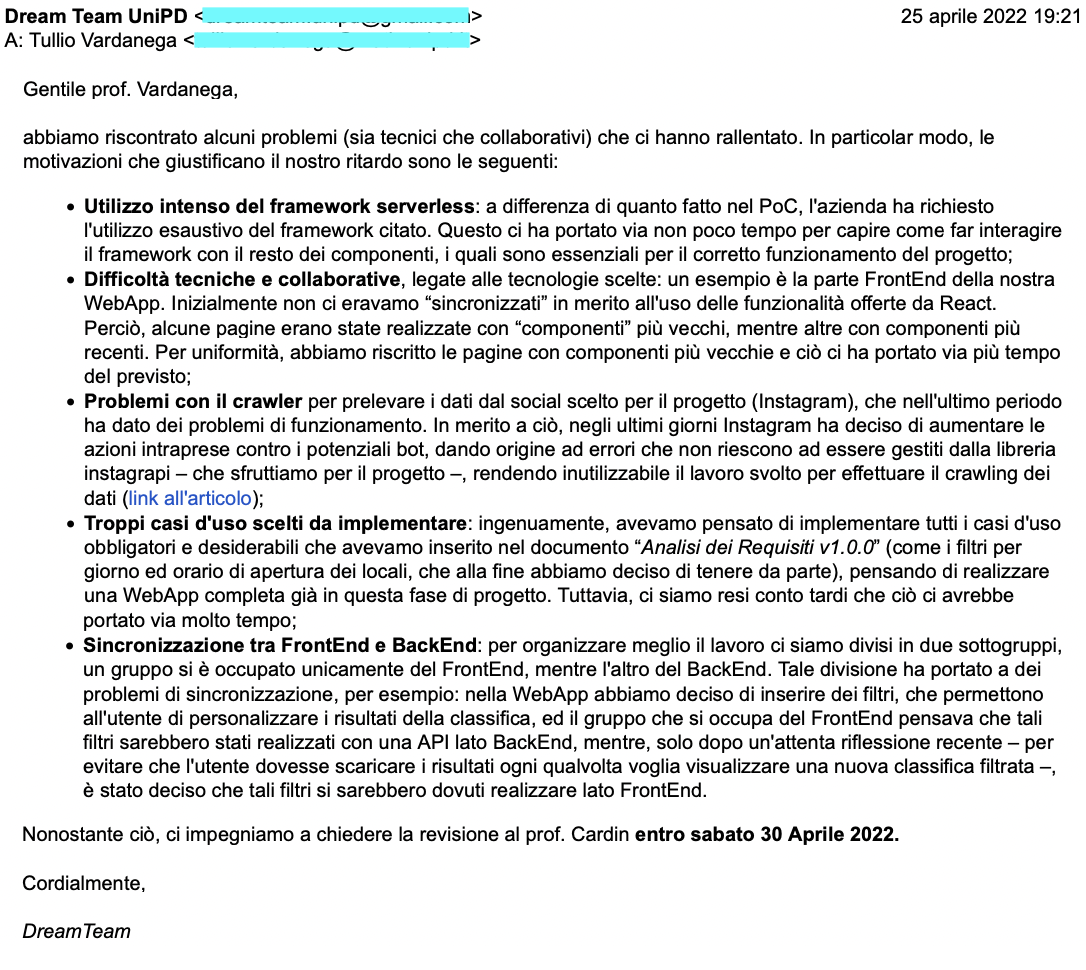
\includegraphics[scale=0.6]{Sezioni/images/copiaemail.png}
\caption{Risposta integrale prof. Vardanega}
\end{figure}

\subsection{Filtri e Likes per la WebApp}

Abbiamo discusso dei filtri per modificare i risultati della classifica (ossia, la pagina “Results”) e dei Likes per inserire o rimuovere un locale dalla lista dei preferiti - sempre dalla pagina dei risultati -; a tal proposito, abbiamo deciso di implementare queste funzionalità per la prossima consegna, in quanto ci siamo resi conto che il relativo sviluppo richiede più tempo del previsto. 


